\documentclass{beamer}
\usepackage[utf8]{inputenc}

\usepackage{appendixnumberbeamer}

\usetheme[sectionpage=progressbar,subsectionpage=progressbar,numbering=fraction,
          progressbar=foot]{metropolis}

\title{Cloud \& Big Data}
\subtitle{Elasticity in Cloud Computing}

\date{\today}
\author{%
  Simon Bihel, \url{simon.bihel@ens-rennes.fr} \\
  Rémi Hutin, \url{remi.hutin@ens-rennes.fr}
}
\institute{%
  University of Rennes I \\
  École normale supérieure de Rennes
}

\begin{document}

\maketitle

\begin{frame}{Table of contents}
  \setbeamertemplate{section in toc}[sections numbered]
  \tableofcontents[hideallsubsections]
\end{frame}


\section{Elasticity: Definition and Differentiation}
\begin{frame}
  \frametitle{What It Is Not~\cite{herbst2013elasticity}}
  \begin{description}
    \parbox{\linewidth}{%
    \item[Scalability] Sustain increasing workloads with adequate performance.
    \item[Efficiency] Amount of resources consumed for a given amount of work.
    }
  \end{description}
\end{frame}

\begin{frame}
  \frametitle{}
  \centering
  \Large\textbf{Elasticity} $\neq$ \textbf{Scalability}

  \visible<2->{It's more than that. That's the selling point.}
\end{frame}

\begin{frame}
  \frametitle{Elasticity~\cite{herbst2013elasticity}~\cite{galante2012survey}~\cite{gulati2011cloud}}
  \begin{definition}
  \parbox{\linewidth}{\textbf{Elasticity} is the degree to which a system is able to adapt to workload changes by provisioning and de-provisioning resources in an autonomic manner, such that at each point in time the available resources \textit{match} the current demand as closely as possible.}
  \end{definition}
\end{frame}

\begin{frame}
  \frametitle{Example of matching demand~\cite{herbst2013elasticity}}
  \begin{figure}
    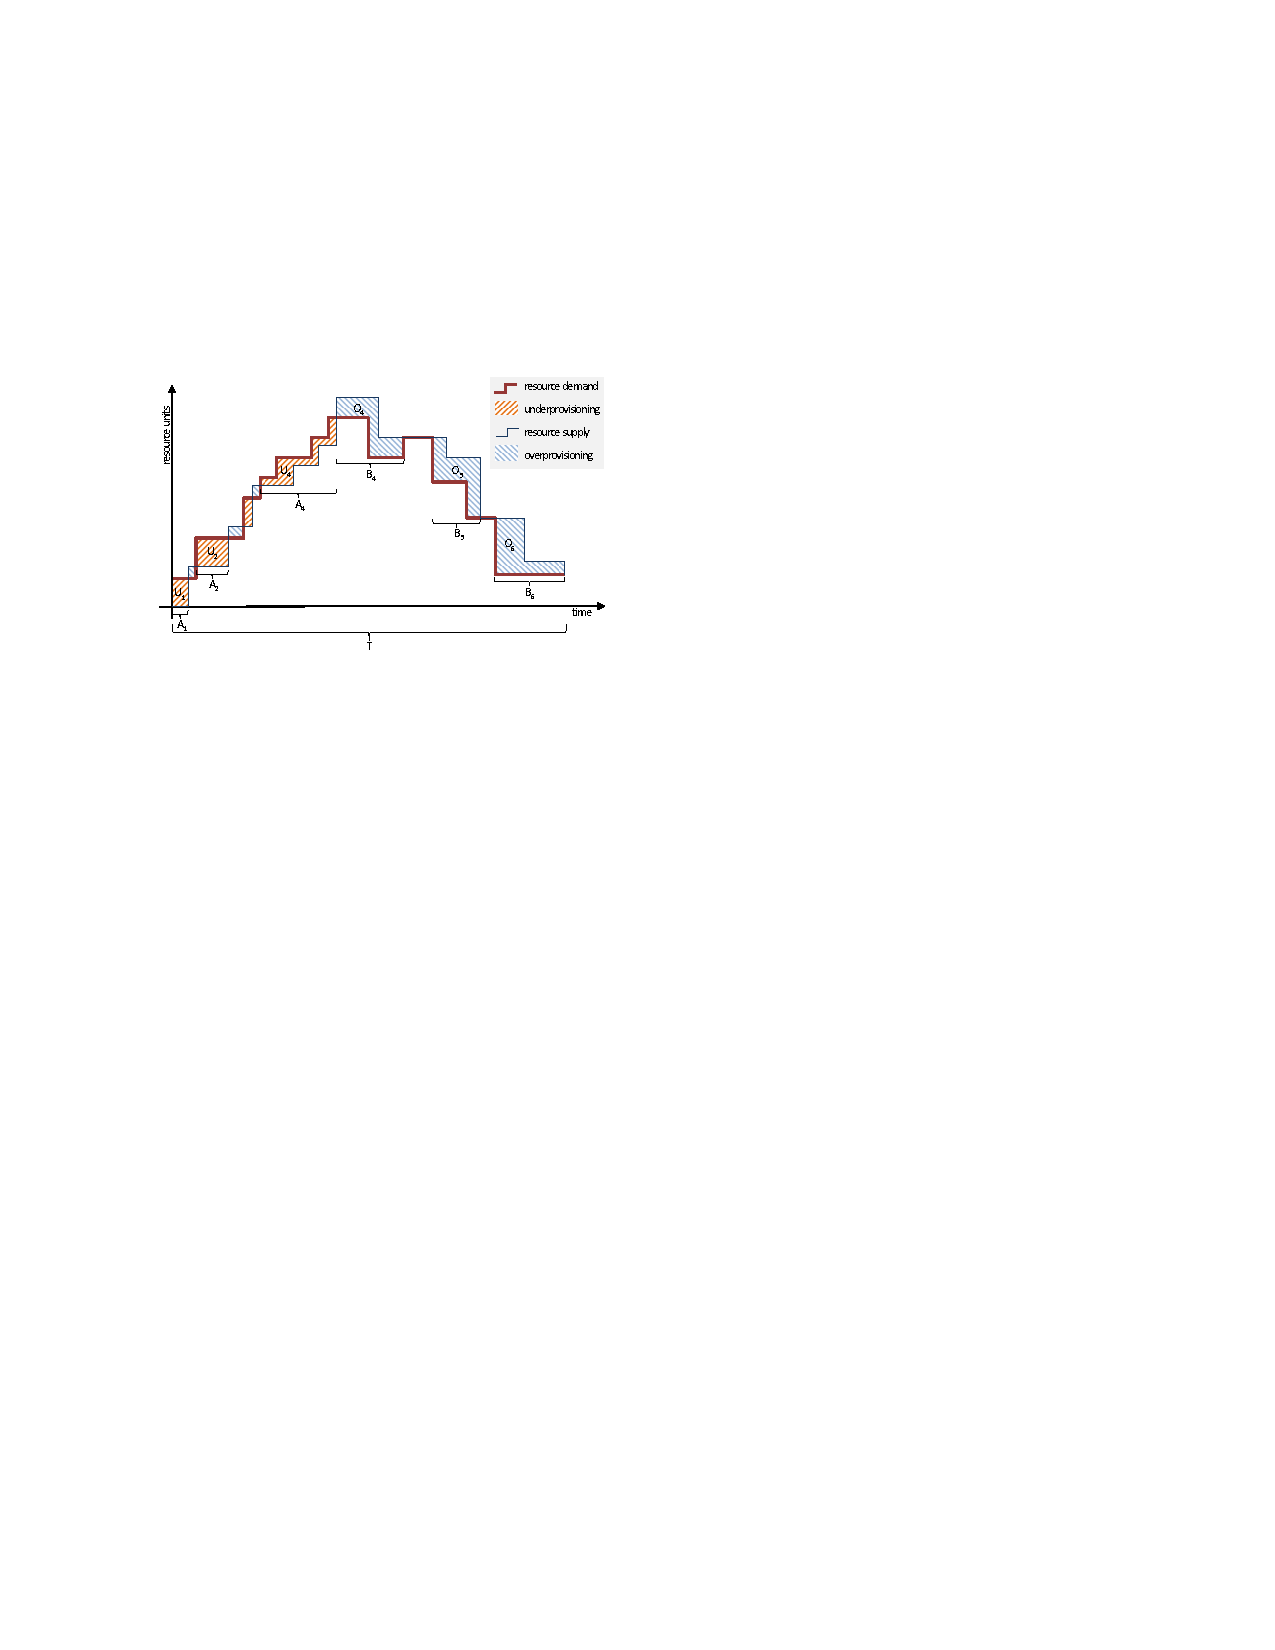
\includegraphics[clip, width=\textwidth]{images/workload}
  \end{figure}
\end{frame}

\begin{frame}
  \frametitle{Different parameters involved in elasticity}
  \includegraphics<1->[width=\textwidth]{images/elasticity2_1}\hspace*{-\textwidth}%
  \includegraphics<2->[width=\textwidth]{images/elasticity2_2}\hspace*{-\textwidth}%
  \includegraphics<3->[width=\textwidth]{images/elasticity2_3}\hspace*{-\textwidth}%
  \includegraphics<4->[width=\textwidth]{images/elasticity2_4}\hspace*{-\textwidth}%
\end{frame}


\section{When to Scale}
\begin{frame}
  \frametitle{Reaction}
  Set of rules (\textit{thresholds}).
\end{frame}

\begin{frame}
  \frametitle{Prediction}
\end{frame}

\begin{frame}
  \frametitle{Example of an elasticity controller~\cite{moore2013coordinated}}
\end{frame}


\section{How to Scale}
\begin{frame}
  \frametitle{Kinds of scaling / Mechanisms}
  \begin{description}
    \item[Horizontal]<1-> (\textit{Replication}) Adding/Removing instances (e.g.\ VMs, modules\dots).
    \item[Vertical]<2-> (\textit{Resizing}) Adding resources (e.g.\ processing, memory\dots).
    \item[Migration]<3-> (\textit{Scaling Out}) Transferring a VM from one physical server to another one.
  \end{description}
\end{frame}

\begin{frame}
  \frametitle{Configurations \& Transitions}
  \vspace*{\fill}
  There is also cost for transition.
\end{frame}

\begin{frame}
  \frametitle{Example of a provisioning system~\cite{sharma2011cost}}
\end{frame}

\begin{frame}
  \frametitle{Example of architecture~\cite{sharma2011cost}}
  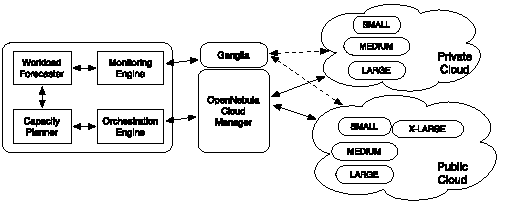
\includegraphics[width=\textwidth]{images/elasticity4_arch.pdf}
\end{frame}


\section*{Conclusion}
\begin{frame}
  \frametitle{Conclusion}
  Not there yet.
  \begin{itemize}
    \item Elements tightly coupled but studied independently.
    \item Mechanisms conceived with assuming other elements in the workflow to be perfect.
  \end{itemize}
\end{frame}


\appendix
\section*{References}
\begin{frame}[allowframebreaks]{References}
  \bibliography{bib}
  \bibliographystyle{abbrv}
\end{frame}


\end{document}
